\documentclass[border=4pt]{standalone}
\usepackage{tikz}
\usetikzlibrary{arrows.meta,positioning,fit,calc,backgrounds}
\usepackage[T1]{fontenc}
\usepackage{lmodern}
\usepackage{amsmath,amssymb}
\definecolor{wsp}{HTML}{2A78D6}
\definecolor{dflt}{HTML}{7A7974}
\definecolor{trn}{HTML}{EB6834}
\definecolor{sb}{HTML}{1BAF7A}
\definecolor{look}{HTML}{6250D6}
\definecolor{ink}{HTML}{0B0B0B}
\definecolor{ink2}{HTML}{52514E}
\definecolor{paper}{HTML}{F4F3EF}
\tikzset{
  box/.style={draw=ink2, rounded corners=3pt, fill=paper, align=center, inner sep=5pt, font=\small, text width=#1},
  box/.default=3.0cm,
  hl/.style={draw=wsp, line width=0.9pt, fill=wsp!8},
  arr/.style={-{Stealth[length=2.2mm]}, line width=0.7pt, draw=ink2},
  note/.style={font=\footnotesize\itshape, text=ink2, align=center},
}

\begin{document}
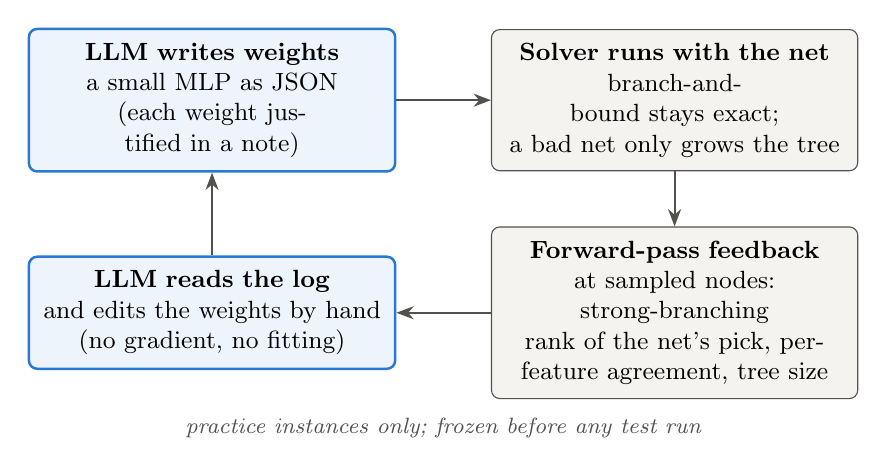
\begin{tikzpicture}[node distance=7mm and 12mm]
\node[box=4.3cm, hl] (llm) {\textbf{LLM writes weights}\\ a small MLP as JSON\\ (each weight justified in a note)};
\node[box=4.3cm, right=of llm] (run) {\textbf{Solver runs with the net}\\ branch-and-bound stays exact;\\ a bad net only grows the tree};
\node[box=4.3cm, below=of run] (diag) {\textbf{Forward-pass feedback}\\ at sampled nodes: strong-branching\\ rank of the net's pick, per-feature agreement, tree size};
\node[box=4.3cm, hl] (read) at (llm |- diag) {\textbf{LLM reads the log}\\ and edits the weights by hand\\ (no gradient, no fitting)};
\draw[arr] (llm) -- (run);
\draw[arr] (run) -- (diag);
\draw[arr] (diag) -- (read);
\draw[arr] (read) -- (llm);
\node[note, anchor=north] at ($(read.south)!0.5!(diag.south)+(0,-0.3)$) {practice instances only; frozen before any test run};
\end{tikzpicture}
\end{document}
